\section{Introduction} \label{introduction}
%% General Introduction
In machine learning applications, a pipeline, a series of complex data processing steps, processes a labeled training dataset and produces a machine learning model.
The model then has to be deployed into a deployment platform where it answers prediction queries in real-time.
To properly preprocess the prediction queries, typically the pipeline has to be deployed alongside the model.

A deployment platform must be robust, i.e., it should accommodate many different types of machine learning models and pipelines.
Moreover, it has to be simple to tune.
Finally, the platform must maintain the quality of the model by further training the deployed model when new training data becomes available.

%% Intro to the problem of continuous improvement
Online deployment of machine learning models is one method for maintaining the quality of a deployed model.
In the online deployment approach, the deployment platform utilizes online learning methods to further train the deployed model \cite{duchi2011adaptive}.
In online learning, the model is updated based on the incoming training data.
Online learning adapts the model to the new training data and provides an up-to-date model.
\deleted[comment={R2:3-Sect1}]{However, purely online deployment approach degrades the quality over time, rendering it ineffective in many cases.}
\added{However, online learning is sensitive to noise and outliers which may result in an increase in the prediction error rate.}
\deleted{In some applications that online learning has proven to be effective,}
\added{Therefore,} to guarantee a high level of quality, one has to tune the online learning method to the specific use case \cite{ma2009identifying, macmahan2013}.
Thus, effective online deployment of machine learning models cannot provide robustness and simplicity.

%Figure \ref{fig:motivational-example} shows the typical process of the existing deployment platforms.
%During the initial training step, a user designs a machine learning pipeline that consists of several data and feature preprocessing steps and trains a machine learning model by utilizing a batch training algorithm.
%Then in the deployment step, the model and the pipeline are deployed into the deployment platform.
%To perform inference, the deployment platform directs the incoming prediction queries through the preprocessing steps.
%Using the preprocessed features, the model makes a prediction.
%During the online update phase, the deployment platform directs the data through the preprocessing steps of the pipeline and then, using an online training algorithm, the platform updates the model.
%Finally, the deployment platform accommodates periodical retraining of the pipeline by either automatically initiating a batch training or prompting the user to train and redeploy a new model to the deployment platform.
%During the periodical retraining, the deployment platform has to disable the online updating of the model.

To solve the problem of degrading model quality, periodical deployment approach is utilized.
In the periodical deployment approach, the platform, in addition to utilizing simple online learning, periodically retrains the deployed model using the historical data.
One of the challenges in many real-world use cases is the size of the training datasets.
Typically, training datasets are extremely large and require hours or days of data preprocessing and training to result in a new model.
Despite this drawback, in some applications, retraining the model is still critical, as even a small increase in the quality of the deployed model can have a large impact.
For example, in the domain of ads click-through rate (CTR) prediction, even a 0.1\% accuracy improvement yields hundreds of millions of dollars in revenue \cite{ling2017model}.
In the periodical deployment approach, while the model is being retrained, new prediction queries and training data are still arriving at the deployment platform.
However, the platform has to answer the prediction queries using the currently deployed model.
Moreover, the platform appends the new training data to the historical data.
By the time the retraining process is over, enough training data is accumulated which requires the deployment platform to perform another retraining.
As a result, the deployed model quickly becomes stale.

Although periodical deployment is robust and easy to tune, it cannot maintain the quality of the deployed model without incurring a high training cost.
We propose a deployment platform that eliminates the need for retraining, thus significantly reducing the training cost while achieving the same level of quality as the periodical deployment approach.
Our deployment platform is robust, i.e., it accommodates many different types of machine learning models and pipelines.
Moreover, similar to the periodical deployment, the tuning process of our deployment platform is simple and requires the same amount of user interaction as the periodical deployment.

%% Use case
%\begin{figure}[h!]
%\centering
%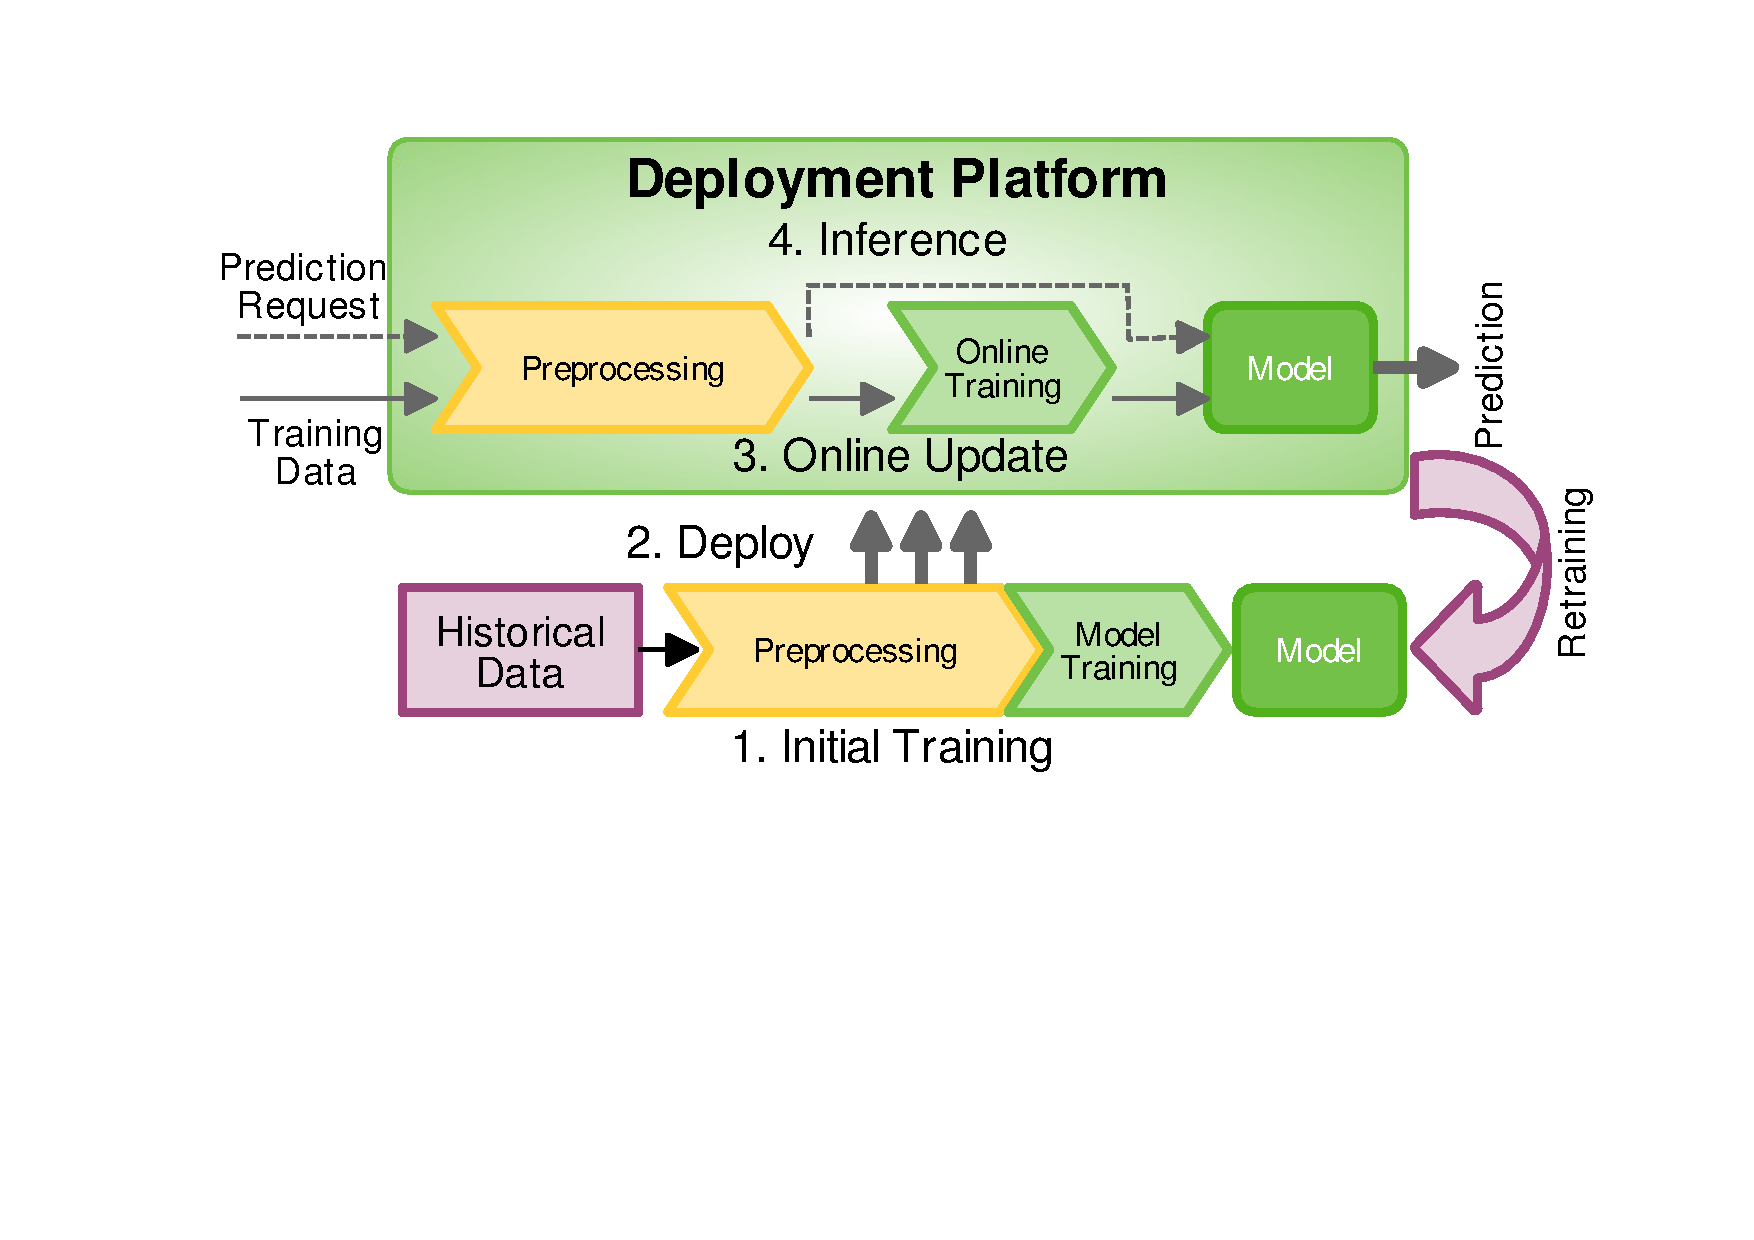
\includegraphics[width=\columnwidth]{../images/generic-motivational-example-v2.pdf}
%\caption{Deployment process of machine learning pipelines}
%\label{fig:motivational-example}
%\end{figure}

%One example is the problem of Ad click prediction \cite{macmahan2013}.
%In Ad click prediction, the machine learning pipeline consists of extracting features from the users and ads. 
%Logistic regression models perform well in this setting \cite{macmahan2013}.
%Prediction queries consist of the user's information and a pool of available ads for displaying to the user.
%Once a prediction is made, a set of ads, with highest prediction scores, are displayed to the user.
%Based on the action of the user (click or no click), new training data will be generated which is sent to the deployment platform for further training of the model.
%Aside from the generated training data, new ads and new users are constantly becoming available.
%As a result, new models have to be periodically trained and redeployed into the deployment platform.

%The above example demonstrates the complexity and suboptimality of the deployment and maintenance of machine learning models and pipelines through periodical retraining.
%Therefore, a flexible deployment platform should meet the model quality requirement without requiring the periodical retraining of the models and pipelines.

%% Our solution
Our deployment platform continuously updates the model using a combination of the historical and incoming training data.
Similar to existing deployment platforms, our platform also utilizes online learning methods to update the model based on the incoming training data.
However, instead of the periodical retraining, our deployment platform performs regular updates to the model based on samples of the historical data.
Our deployment platform offers the following two features:

\textit{Proactive training.}
Proactive training is the process of utilizing samples of the data to update the deployed model.
First, the deployment platform processes a given sample using the pipeline, then it computes a partial gradient and updates the deployed model based on the partial gradient.
The updated model is immediately ready for answering prediction queries.
Our experiments show that proactive training reduces the training time by one order of magnitude while providing the same level of quality when compared to the periodical deployment approach.

\textit{Online Statistics Computation and Dynamic Materialization.}
Before updating the model using proactive training, the pipeline has to preprocess the training data.
Every component of the pipeline needs to scan the data, updates the statistics (for example the mean and the standard deviation of the standard scaler component), and finally, transform the data.
Computing these statistics and transforming the data are time consuming processes.
Aside from the proactive training, our deployment platform also employs online learning methods to update the model in real-time.
During the online learning, we compute the required statistics and transform the data.
The deployment platform stores the updated statistics for every pipeline component and materializes the transformed features by storing them in memory or disk.
In presence of a limited storage capacity, the platform removes the older transformed features, and only re-materializes them when needed (through a process called \textit{dynamic materialization}).
By reusing the computed statistics and the materialized features during the proactive training, we eliminate the data preprocessing steps of the pipeline and further decrease the proactive training time.

% Our contributions
In summary, our contributions are:
\begin{itemize}
\item A platform for continuously training deployed machine learning models and pipelines that adapts to the changes in the incoming data. The platform accommodates different types of machine learning models and pipelines. In our experiments, we design and deploy two different machine learning pipelines.
\item Proactive training of the deployed models and pipelines that frequently updates the model using samples of the data which \added[comment={R2: 6}]{completely eliminates the need for periodical retraining while providing the same level of model quality.} \deleted{guarantees high-quality models while completely eliminating the need for periodical retraining.}
\item Efficient pipeline processing and model training by online statistics computation and dynamic materialization, \added[comment={R2:6}]{which provides} \deleted{thus guaranteeing the availability of} up-to-date models for answering prediction queries.
\end{itemize}

The rest of this paper is organized as follows:
In Section \ref{background}, we provide background information on the optimization strategy we utilize in our continuous deployment platform and tuning mechanism of the existing deployment platforms.
Section \ref{continuous-training-serving} describes the details of our continuous training approach.
In Section \ref{sec:system-architecture}, we introduce the architecture of our deployment platform.
In Section \ref{evaluation}, we evaluate the performance of our continuous deployment platform.
Section \ref {related-work} discusses the related work.
Finally, Section \ref{conclusion} presents our conclusion and the future work.